%*****************************************
\chapter{Ergebnisse}\label{ch:results}
%*****************************************
\newcommand{\lo}{\enquote{llama$2$\_$0$e}}
\newcommand{\liv}{\enquote{llama$2$\_$1$e\_v$100$}}
\newcommand{\lia}{\enquote{llama$2$\_$1$e\_a$30$}}
\newcommand{\lev}{\enquote{llama$2$\_$3$e\_v$100$}}
\newcommand{\lea}{\enquote{llama$2$\_$3$e\_a$30$}}
\newcommand{\lsa}{\enquote{llama$2$\_$5$e\_a$30$}}
\newcommand{\lioa}{\enquote{llama$2$\_$10$e\_a$30$}}

In dieser Arbeit wurde die Konzeptionierung und Durchführung eines Continual Pretraining von Llama Modellen beschrieben.
Diese Modelle wurden anschließend nach den in \cref{sec:approach:comparison} genannten Kriterien Korrektheit, Erklärbarkeit, Fragenverständnis und Robustheit verglichen.
Die Durchführung dieses Vergleichs ist in \cref{sec:evaluation} gezeigt.
In diesem Kapitel werden die Ergebnisse vorgestellt und analysiert, wobei auch hier eine Unterteilung nach den Kriterien vorgenommen wird.
Zu vergleichende Modelle sind GPT4,
Llama 2 7B untrainiert (in den Grafiken als \lo bezeichnet),
Llama 2 7B auf 1 Epoche mit 4 Nvidia Tesla V100 Grafikkarten trainiert (in den Grafiken als \liv bezeichnet),
Llama 2 7B auf 1 Epoche mit 4 Nvidia Tesla A30 Grafikkarten trainiert (bezeichnet als \lia),
Llama 2 7B auf 3 Epochen mit 4 Nvidia Tesla V100 Grafikkarten trainiert (bezeichnet als \lev),
Llama 2 7B auf 3 Epochen mit 4 Nvidia Tesla A30 Grafikkarten trainiert (bezeichnet als \lea),
Llama 2 7B auf 5 Epochen mit 4 Nvidia Tesla A30 Grafikkarten trainiert (bezeichnet als \lsa) und
Llama 2 7B auf 10 Epochen mit 4 Nvidia Tesla A30 Grafikkarten trainiert (bezeichnet als \lioa).



\section{Analyse Korrektheit}\label{sec:results:correctness}
\subsection{Vergleich totaler Zahlen}
\begin{figure}
    \makebox[\textwidth][c]{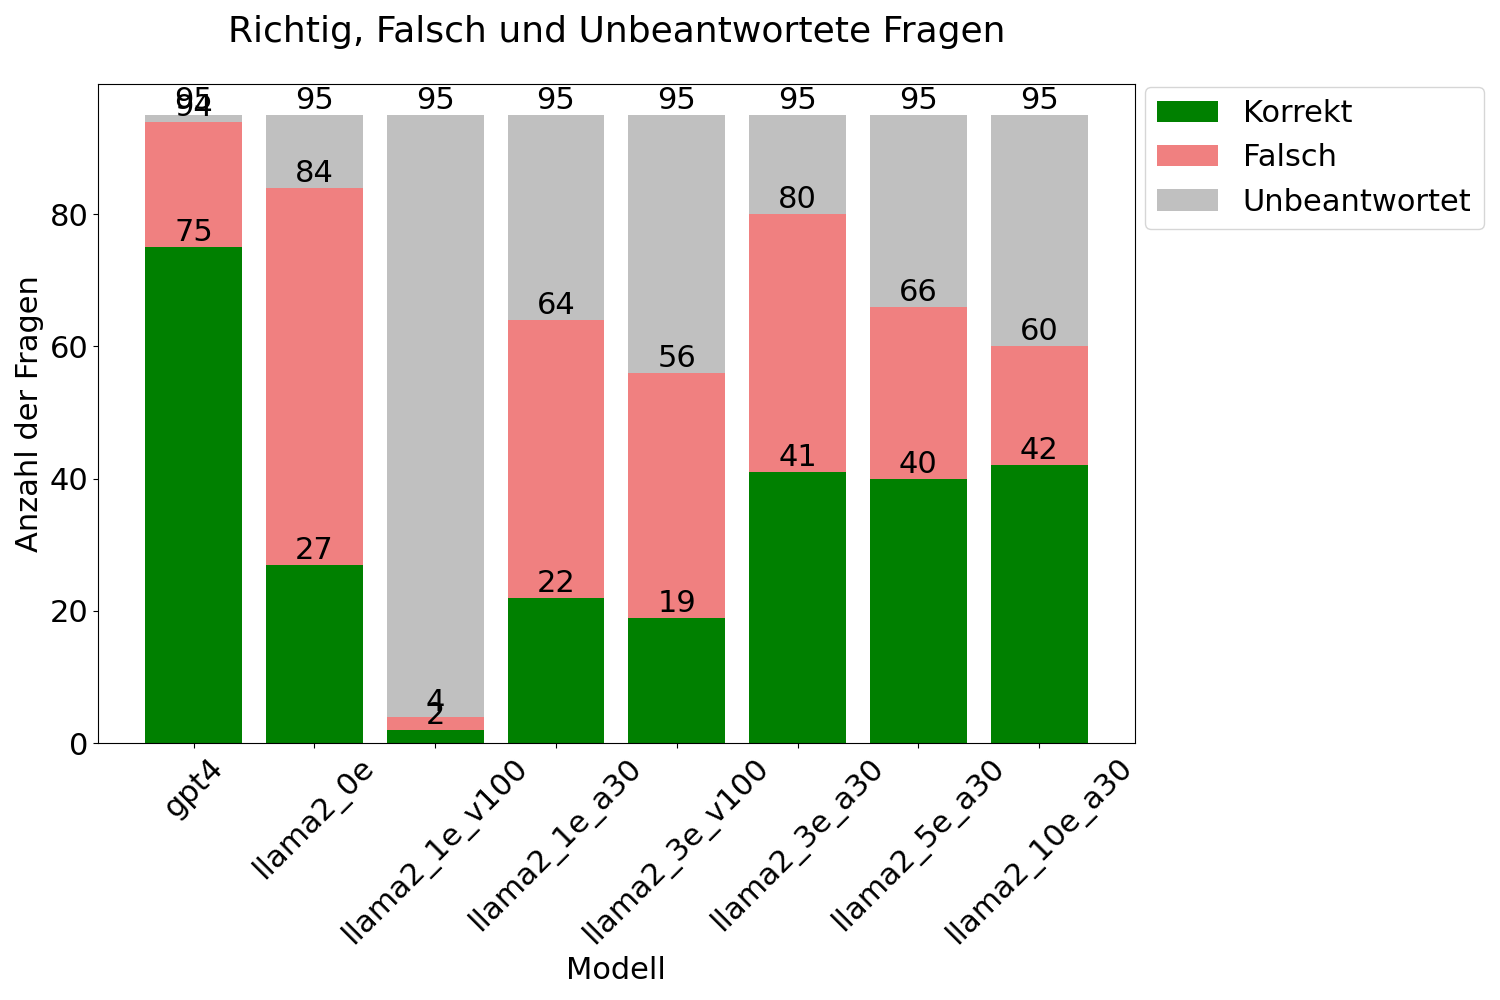
\includegraphics[width=1.2\textwidth]{results/answers_total.png}}
    \caption{Vergleich verschiedener Modelle und ihren totalen Leistungen bei der Beantwortung von Fragen.}
    \label{fig:results:answers_total}
\end{figure}
\cref{fig:results:answers_total} zeigt die Aufteilung der korrekt, falsch und unbeantworteten Fragen der evaluierten Modelle.
Alle Modelle erhielten die selben $95$ Fragen mit identischem Kontext.
Diese absoluten Zahlen zeigen eine grobe Tendenz der Leistungen, widerspiegeln jedoch die wahren Leistungen nicht.
Eine Frage gilt als richtig beantwortet, wenn mindestens eine richtige Antwort gegeben wurde.
Dies führt zu missverständlich guten Ergebnissen.
Dennoch ist klar zu erkennen, dass GPT4 einen deutlichen Vorsprung gegenüber den Llama Modellen hat.
Das untrainierte Llama Modell beantwortete \SI{28}{\percent} der Fragen mit mindestens einer korrekten Antwort, konnte jedoch ebenso einen Großteil der Fragen beanworten und liefert bei \SI{11}{\percent} keine Antwort.\\

Das \liv-Modell liefert mit \SI{2}{\percent} die wenigsten korrekten Antworten und zeigt ein generelles Verlernen grundlegender sprachlicher Fähigkeiten.
Im Gegenzug zeigt das \lia-Modell eine vergleichbare, wen auch etwas schlechtere Leistung als das untrainierte Modell.\\

Mit dem \lev-Modell konnte eine deutliche Leistungssteigerung gegenüber einer Epoche erreicht werden, jedoch ist die Gesamtleistung bleibend schlechter als das untrainierte Modell.
Das \lea-Modell übertraf dafür erstmalig die Leistungen des untrainierten Modells und beantwortete \SI{43}{\percent} der Fragen mit mindestens einer korrekten Antwort.\\

Modelle mit höherer Epoche wurden außschließlich auf A30 Grafikkarten trainiert und zeigten keine weitere Leistungssteigerung, beantworteten jedoch stetig weniger Fragen.
Hier ist eine Präferenz von keiner Antwort gegenüber einer falschen Antwort zu erkennen.\\

\subsection{Stärken und Schwächen der Modelle}
Zusätzlich zur Gesamtleistung der Modelle fand auch eine Unterteilung in Fragetypen und Fragequellen statt.
Ähnliche Grafiken wie aus \cref{fig:results:answers_total} sind im Anhang enthalten.
Unterschiedene Fragetypen sind Singulär-Fakt Fragen (bezeichnet als \enquote{single}), Multi-Fakten Fragen (bezeichnet als \enquote{multi}) und Transfer-Fragen (bezeichnet als \enquote{transfer}). Unterschiedene Fragequellen sind das Buch \enquote{Health Information Systems} von \citet{bb} (bezeichnet als \enquote{book}), mündliche Klausurfragen aus dem Modul \enquote{Architektur von Informationssystemen im Gesundheitswesen} vom Jahr 2021 (bezeichnet als \enquote{A\_2021}), schriftliche Klausurfragen aus dem Modul \enquote{Informationssysteme in medizinischer Versorgung und Forschung} vom Jahr 2022 (bezeichnet als \enquote{IS\_2022\_07\_18}) und schriftliche Klausurfragen aus der Nachholklausur des Moduls \enquote{Informationssysteme in medizinischer Versorgung und Forschung} vom Jahr 2022 (bezeichnet als \enquote{IS\_2022\_09\_27}).\\

Das GPT4 Modell besitzt keine Präferenz gegenüber Fragetypen, beantwortete jedoch Fragen aus dem Buch deutlich besser mit \SI{93}{\percent} korrekten Antworten.
Vergleichsweise wenige Antworten wurden bei beiden schriftliche Klausuren gegeben, wobei die Klausur \enquote{IS\_2022\_07\_18} besonders wenig Fragen enthielt und daher keine genauen Angaben möglich sind.\\

Das untrainierte Llama Modell zeigte eine eindeutige Stärke bei Multi-Fakten Fragen mit \SI{39}{\percent} richtigen Antworten und konnte \SI{27}{\percent} der mündlichen Klausurfragen beanworten. 
\subsection{Verbesserungen durch Training}
\subsection{Vergleich MakroF1}
\todo{results/makro\_total.png fehlt im Repo}
\begin{figure}
    \makebox[\textwidth][c]{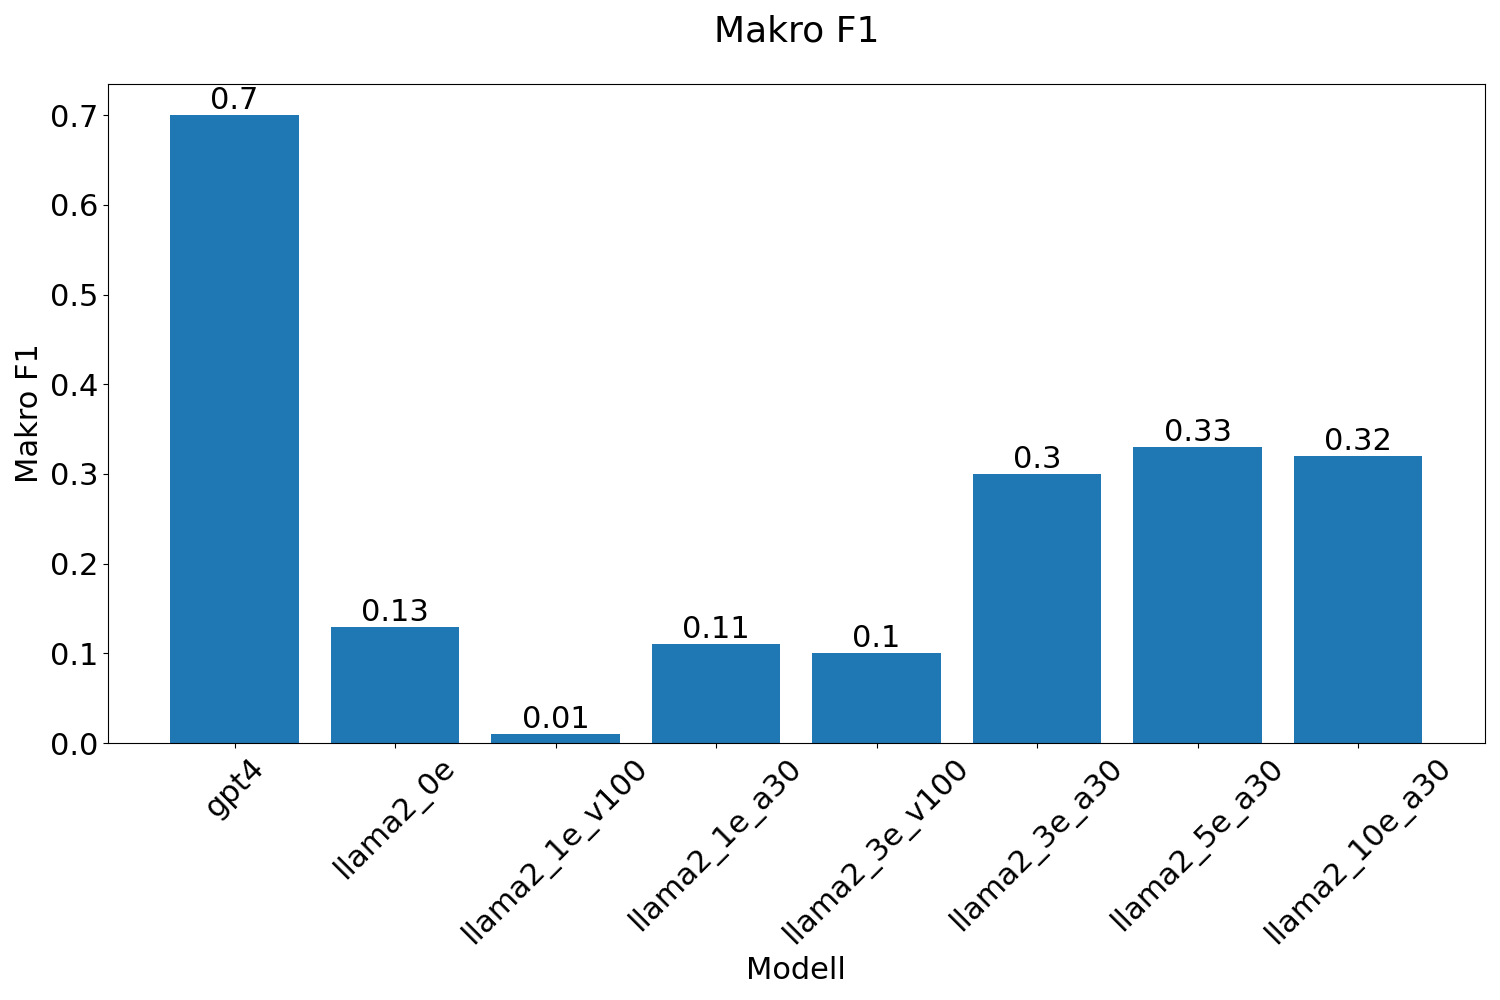
\includegraphics[width=1.2\textwidth]{results/makro_total.png}}
    \caption{Vergleich verschiedener Modelle und Makro F1 Werten bei der Beantwortung von Fragen.}
    \label{fig:results:makro_total}
\end{figure}
\subsection{Zusammenfassung}
\section{Analyse Erklärbarkeit}\label{sec:results:explainability}
\section{Analyse Fragenverständnis}\label{sec:results:questionunderstanding}
\section{Analyse Robustheit}\label{sec:results:robustness}
\section{Zusammenfassung}\label{sec:results:summary}

% Stärken von GPT4
% Keine Präferenz in Fragentyp
% Kann Fragen des Buches deutlich besser beantworten 93%

% Schwächen von GPT4
% keine eindeutige Schwäche bei Fragentyp
% IS_2022_07_18: 55% (wenig fragen)
% IS_2022_09_27: 70% (wenig fragen)

% Stärken von LLaMA untrainiert
% Multi-Fakt Fragen (2x mehr als andere Typen, 39\%)
% IS 2022_07_18 55% richtig, aber wenig Fragen - keine genauen Angaben möglich
% A_2021: 27%

% Schwächen von LLaMA untrainiert
% Single  20\%  & Transfer 21% -richtig beantwortet
% Andere Sources:
% IS_2022_09_27: 25%
% Book_ 24%

% Stärken von LLaMA v100 1 Epochen
% generell Schlecht

% Schwächen von LLaMA v100 1 Epochen
% ---

% Stärken von LLaMA a30 1 Epochen
% Multi 36%
% A2021: 40%

% Schwächen von LLaMA a30 1 Epochen
% Single: 5%
% IS_2022_09_27: 12%


% Stärken von LLaMA v100 3 Epochen
% Transfer Fragen: 26%
% IS_2022_09_27: 22%

% Schwächen von LLaMA v100 3 Epochen
% Single Fakt Fragen: 17%
% A_2021: 13%

% Stärken von LLaMA a30 3 Epochen
% Transfer: 52%
% A_2021: 54%

% Schwächen von LLaMA a30 3 Epochen
% Single: 32%
% IS_2022_09_27: 32%

% Stärken von LLaMA a30 5 Epochen
% Multi: 52%
% Book: 63%

% Schwächen von LLaMA a30 5 Epochen
% Single: 26%
% IS_2022_09_27: 19%

% Stärken von LLaMA a30 10 Epochen
% Multi: 47%
% Book: 60%

% Schwächen von LLaMA a30 10 Epochen
% Transfer: 26%
% IS_2022_09_27: 25% (IS_2022_07_18: 22% (wenig fragen))

% Vergleich LLaMA mit GPT4 durchgängig bessere Ergebnisse bei allen Fragenarten
% Vergleich LLaMA v100 1 Epoche mit anderen Modellen durchgängig schlechtere Ergebnisse bei allen Fragenarten
% Vergleich LLaMA a30 1 mit LLaMA 0:
% - minimal Verbesserung transfer
% - Vergleichbar Multi
% - Schlechter Single
% - generell mehr Fragen unbeantwortet
% - Besser bei A_2021
% - Schlechter bei IS_2022_09_27, IS_2022_07_18 und Book
% - Deutlich mehr unbeantwortet bei IS_2022_09_27 und IS_2022_07_18

% Vergleich LLaMA v100 3 mit LLaMA 0:
% - Minimale Verbesserung bei Transfer Fragen
% - Wesentlich mehr unbeantwortete Fragen bei Singulär
% - Wesentlich mehr unbeantwortete Fragen bei Multi-Fakt
% - Vergleichbar bei IS_2022_09_27 und Book
% - Schlechter bei A_2021 und IS_2022_07_18
% - A2021, IS_2022_09_27 wesentlich mehr unbeantwortet

% Vergleich LLaMA a30 3 mit LLaMA 0:
% - Verbesserung bei Transfer und Single
% - kleine Verbesserung bei Multi
% - Alle Fragen bei transfer verstanden
% - Leicht weniger Fragen beantwotet bei single und Multi
% - Verbesserung Book und A2021
% - Leichte Verbesserung bei IS_2022_09_27
% - Verschlechterung bei IS_2022_07_18
% - Mehr beantwortet bei Book
% - Weniger beantwortet bei A_2021

% Vergleich a30 3 mit a30 1:
% - Verbesserung bei allen Typen
% - Verbesserung bei allen Sources außer IS_2022_07_18
% - mehr Fragen beantwotet bei allen Typen
% - Mehr fragen beantwotet bei allen Sources außer A_2021

% Vergleich a30 3 mit v100 3:
% - Verbesserung bei allen Typen
% - mehr Fragen beantwortet bei allen Typen
% - Verbesserung bei allen Sources
% - Mehr Fragen beantwortet bei allen Sources außer IS_2022_07_18

% Vergleich a30 5 mit Llama 0:
% - Verbesserung bei allen Typen
% - Weniger Fragen Beantwotet bei allen Typen
% - Verbesserung bei A_2021 und Book
% - Verschlechterung bei IS_2022_09_27 und IS_2022_07_18
% - Mehr fragen beantwortet bei Book
% - Weniger Fragen beantwortet bei allen Sources außer Book

% Vergleich a30 5 mit a30 3:
% - Verbesserung bei Multi
% - Verschlechterung bei Single, Transfer
% - Weniger Fragen beantwortet bei allen Typen
% - Verbesserung bei Book
% - Verschlechterung bei allen Sources außer Book
% - Weniger Fragen beantwotet bei allen Sources außer Book

% Vergleich a30 10 mit Llama 0:
% - Verbesserung bei allen Typen
% - Weniger Fragen beantwortet bei allen Typen
% - Verbesserung bei A_2021 und Book
% - Verschlechterung bei IS_2022_07_18
% - Weniger Fragen beantwortet bei allen Sources

% Vergleich a30 10 mit a30 3:
% - Vergleichbar bei allen Typen
% - Mehr Fragen beantwortet bei Multi
% - Weniger Fragen beantwortet bei Transfer
% - Besser bei Book
% - Schlechter bei IS_2022_09_27, IS_2022_07_18
% - Weniger Fragen beantwortet bei allen Sources außer A_2021

% Vergleich a30 10 mit a30 5:
% - Besser bei single
% - Mehr bei Multi
% - Weniger bei Transfer, Single
% - Besser bei IS_2022_09_27
% - Mehr bei A2021
% - Weniger bei allen außer A2021

% Ranking - Richtig Beantwortet:
% - GPT4 immer besser
% - 10e, 5e, 3e a30 besten Ergebnisse
% - v100 1e schlechteste Ergebnisse

% Ranking Beantwortet:
% - GPT4, llama0, llama 3e
% - v100 1e schlechteste Ergebnisse

% Ranking MakroF1:
% - GPT4 besstes
% - A30 3e, 10e und 5e sehr gut
% - 5e und 10e durch Book
% - v100 1e schlechteste Ergebnisse


% Analyse der Korrektheit
% - Betrachtung der MakroF1 Werte bestätigt totale Anzahl der Fragen Ergebnisse
% - GPT4 erreicht 0.7 MakroF1, vergleichbar mit ERgebnissen aus GPT4 Paper (Medical Knowledge)
% - LLaMA auch im untrainierten Zustand deutlich unter normaler Leistung
% - Doppelte Leistung von untrainiert durch 5e, 10e und 3e erreicht
% - 1e vergleichbar mit 0e
% - insbesondere Transfer-Fragen besser
% - synthetische gute Ergebnisse bei 5e, 10e durch overfitting auf Buchfragen
% - 3e erreicht gute Ergebnisse bei A2021 -> kann dadurch mithalten

% Begründung der Ergebnisse
% - GPT4 durch Größe unschlagbar
% - hier nur mit LLaMA 7B verglichen, zu erwarten bei größere Modelle deutlich bessere Leistung
% - Verlauf des Trainings einschätzbar: 1 Epoche deutlich zu wenig, so gut wie keine Leistungssteigerung
% - temporäres Overfitting an Formattierungsarten (Überschriften, Aufzählungen)
%     hier Beispiel von LLaMA 1 einfügen
% - Overfitting durch identische Antwortimitierung bei 5e und 10e
%     hier Beispiel 10e einfügen
% - Maximale Leistung bei 3e/5e erreicht, 10e keine Verbesserung
% - generell sehr wenig Trainigsdaten (600kB), Gefahr des overfittings nach 3 Epochen existent
% - weitertrainieren von v100 nicht möglich, beschrieben in Kapitel 5
% - V100 FP16 training führt zu deutlich schlechteren Leistungen
% - LLaMA erlernt keine falschen Fakten, deutlich mehr Fragen unbeantwortet, während LLaMA 0 mehr Fragen falsch beantwortet
%     - steigert sich mit steigender Epoche -> anzeichen für Overfitting

% - Tatsächliche Steigerung bei Transfer-Fragen
% Ergebnisse enthalten jedoch gravierende Formattierungs- und Wiederholungsfehler

% Modelle im aktuellen Zustand nicht nutzbar, da kein Endtoken für Antworten vorhanden
%     hier Beispiel von LLaMA 5e einfügen


% Analyse Erklärbarkeit
% - GPT 4 auch hier unschlagbar, nahezu jede Antwort enthält Erklärung, 97%
% - LLaMA 0, V100 3, a30 1 unbeeinflusst bei 50% der Fragen
% - LLama 3e, 5e, 10e deutlich besser 85% der Fragen
% - Ergebnisse unabhängig von Source oder Type
% - Verbesserung durch Human Reinforcement Training möglich, um Erklärungen zu belohnen (nicht existent im Trainingsdatensatz)

% Analyse Fragenverständnis
% - Fragenverständnis nicht äquivalent zu "Fragen beantwortet"
% - Fragenverständis bei LLaMA 0 nur durch a30 3 geschlagen (64%, 72%)
% - Ansonsten starker abfall, V100 3 nur noch bei 40%
% - GPT4 versteht so gut wie jede Frage (97%)
% - Multi Fragen bessere Leistung von Llama0 (81%), Andere Modelle bei 63%, begründet durch Leistungsabfall bei A_2021 Fragen
% - IS Fragen zeigen deutliche Leistungssteigerung und abnahme (zu wenig vs zu viel trainiert)


% Analyse Robustheit
% - Rechtschreibfehler führen zu falschen Antworten
% - LLaMA 0 profitiert etwas durch Fehler, erhöhter MakroF1 Wert (vollständigere Antworten)
% - Auch GPT4 schwierigkeiten bei Transfer
% - Andere Modelle Leistungsabfall um ungefähr 50%

% - Rechtschreibfehler in Fachbegriffen erschweren Faktenwiedergabe, da Tokenization Wörter anders
% unterteilt (teilweise auch in einzelne Buchstaben)
% - schlechtere Leistungen zu erwarten gegenüber ohne Fehler
% - zeigt generelles Verständnis von Fakten unabhängig von Textrepräsentation
% - LLaMA 0 enthaltenes Wissen durch größere Datenmengen fundierter
% - LLaMA 3e, 5e, 10e durch einzelnens Buch (wenig Daten) erst oberflächliche Wissensaneignung
% - scheint teile des LLaMA 0 Wissens ersetzt / versteckt zu haben

% Gesamtanalyse
% - LLaMA kommt nicht an Leistungen von GPT4
% - Trainingsart entscheident (v100 schlechter als Llama 0)
% - Beste Leistungen zwischen a30 3 Epochen und a30 5 Epochen
% - Ab 5 Epochen Overfitting Status -> Überaus gut bei Buchfragen, andere Fragen schlechter
% - Präferenz von Keiner Antwort gegenüber einer Antwort wird mit steigender Epoche deutlicher

% - Erklärbarkeit und Fragenverständnis ebenso unter GPT4-
%     - deutliche Verbesserung ab a30 3 Epochen erreicht
%     - zeigt wahre Leistung von 3 Epochen gegenüber 5 und 10 Epochen
% - Robustheit zeigt, dass Wissen oberflächlich erlernt wurde, jedoch nicht fundiert verankert ist
%     - Wird nicht besser mit längerem Training
%     - Overfitting wirkt entgegen Robustheit

% Leistungssteigerung möglich durch:
% - Größere Modelle generelle Verbesserung zu erwarten (LLaMA 13B, 33B)
% - Mehr Trainingsdaten
%     - sinkt Gefahr des overfittings
%     - Wissen wird fundierter erlernt, da in unterschiedlicher Formulierung enthalten
% - Leistungssteigerung durch Human Reinforcement Learning
%     - bessere Erklärbarkeit zu erwarten


